% !TEX encoding = UTF-8
% !TEX TS-program = pdflatex
% !TEX root = ../tesi.tex
% !TEX spellcheck = it-IT

%**************************************************************
\chapter{Analisi dei requisiti}
\label{cap:analisi-requisiti}
%**************************************************************

Sin dalla sua concezione, la piattaforma Plot è stata pensata come un prodotto unico e fatto su misura per il cliente. Questo ha impedito la definizione di una struttura di base sulla quale innestare eventuali cambiamenti. \\
La prima attività del progetto è stata dunque la consultazione dello schema del database e del codice relativo al \gls{cms}\glsfirstoccur{} di Plot 1.0. Successivamente sono state intervistate le persone coinvolte nello sviluppo di Plot 1.0: developer, responsabili dei contenuti ed utilizzatori del \gls{cms}\glsfirstoccur{} in modo da capire cosa non li soddisfacesse nella struttura attuale e cosa potesse essere fatto per migliorarla.
Da queste interviste sono stati sintetizzati i requisiti che il database ed il \gls{cms}\glsfirstoccur{} avrebbero dovuto avere. Tali requisiti sono stati fondamentali per la successiva progettazione ma possono risultare utili anche all'azienda per valutare in modo più razionale limiti e possibilità della piattaforma.

\section{Requisiti del database}
\subsection{Descrizione dei requisiti}
Un \textbf{consumer} è un concetto astratto che rappresenta un generico utilizzatore della piattaforma Plot, esso è caratterizzato da nome, cognome, email e password.
Un consumer può concretizzarsi nel concetto di admin o user. \\
Un \textbf{admin} rappresenta un amministratore del \gls{cms}\glsfirstoccur{}, ha quindi l'autorizzazione di accedere al \gls{cms}\glsfirstoccur{} ma non può accedere alla parte di gioco. \\ 
Uno \textbf{user} rappresenta un utente del gioco e può quindi accedere alla parte di gioco ma non al \gls{cms}\glsfirstoccur{}. \\
Solitamente i consumer si autenticano presso la piattaforma tramite email e password ma può capitare che gli user utilizzino un servizio di autenticazione esterno tramite \textit{token}.
\\ \\
Un \textbf{invitation} rappresenta un invito che può essere spedito o ricevuto da uno user durante la fase di inviti. Un invitation è caratterizzato dal mittente e dal destinatario, che dovranno essere entrambi user.
\\ \\
Terminata la fase di inviti, ogni user appartiene ad un \textbf{team} caratterizzato da un nome e da un'immagine rappresentativa dello stesso. I team vengono creati a priori e sono associati agli user solo al termine della fase di inviti. 
\\ \\
Qualsiasi richiesta \gls{http}\glsfirstoccur{} effettuata da uno user nel front end di gioco genera un \textbf{log} contenente:
\begin{itemize}
	\item Un riferimento allo user che ha effettuato la richiesta;
	\item Indirizzo IP del dispositivo che ha effettuato la richiesta;
	\item Il metodo \gls{http}\glsfirstoccur{} utilizzato per la richiesta;
	\item L'\gls{url}\glsfirstoccur{} al quale è stata inoltrata la richiesta;
	\item Lo user agent che ha effettuato la richiesta;
	\item Eventuali dati aggiuntivi trasportati dalla richiesta.
\end{itemize}  

Un \textbf{language} rappresenta una lingua parlata ed è caratterizzato da un nome (es. Italiano) e da un codice identificativo (es. it). \\
Una \textbf{translation} rappresenta una traduzione disponibile per un certo contenuto in un particolare language.
Ogni user può indicare il proprio language preferito e questa informazione può essere utilizzata per fornire i contenuti di gioco localizzati in base allo user. \\
Ogni contenuto traducibile deve prevedere un testo di default da utilizzare nel caso in cui non siano state previste traduzioni per la lingua scelta dallo user.
\\ \\
Uno user può appartenere ad una \textbf{category}, il significato della category non è fissato a priori ma può essere istanziato in base alle necessità del progetto e del cliente che lo richiede. Il concetto di category è quindi astratto e viene utilizzato per partizionare gli user sulla base di una o più caratteristiche.  
Ad esempio, gli user possono essere categorizzati per regione di appartenenza o per posizione lavorativa. Una category ha un nome che la identifica. \\
Per questo progetto vengono istanziate le due category più usate nei Plot passati: region e business role.\\
Una \textbf{region} rappresenta l'area del mondo alla quale appartiene un certo user ed è caratterizzata da una timezone. Una \textbf{timezone} identifica un particolare fuso orario ed è caratterizzata dal nome (es. Central European Time), dal codice identificativo della timezone (es. CET) e dall’offset rispetto allo UTC (es. +1).
Una region può quindi rappresentare un insieme di stati, un singolo stato o una porzione di esso, questo dipende dallo specifica istanza di Plot.\\
Un \textbf{business role} rappresenta il ruolo dello user all'interno dell'azienda o, più in generale, l'area lavorativa alla quale esso afferisce.
\\ \\
Un Plot è composto da una o più \textbf{mission}. Ogni mission è caratterizzata da un nome, un'immagine rappresentativa, una data d'inizio e una data di fine, oltre la quale la mission si considera chiusa.
Una mission è composta da più \textbf{post}. Ogni post prevede un testo ed appartiene ad una delle seguenti tipologie: 
\begin{itemize}
	\item \textbf{Text post};
	\item \textbf{Captcha post}: prevede una domanda indirizzata ai singoli user;
	\item \textbf{Team post}: prevede una domanda indirizzata ai team. 
\end{itemize}

Una \textbf{question} è un concetto astratto che rappresenta una generica domanda, essa prevede un testo che riporta il corpo della domanda stessa. Una question può essere istanziata da una user question o da una team question.\\
Una \textbf{user question} rappresenta una domanda indirizzata ai singoli user. Le user question sono caratterizzate dalle category alle quali sono rivolte. Se il concetto di category è utilizzato dalla particolare istanza di Plot, è possibile assegnare domande diverse a user appartenenti a diverse category. Viceversa, se il concetto di category non è utilizzato, ogni domanda può potenzialmente essere assegnata ad ogni user.
Una user question è visibile alla pubblicazione del captcha post al quale appartiene.\\
Una \textbf{team question} rappresenta una domanda indirizzata ai team. Le team question prevedono un tempo limite entro il quale devono ricevere risposta. Qualsiasi componente del team può fornire una o più risposte ad una specifica domanda.
Una team question non è immediatamente visibile alla pubblicazione del team post al quale appartiene, per svelarla è necessario che un componente del team dichiari di volerla visualizzare, a quel punto la domanda è visualizzabile da tutti i membri del team. Nel momento in cui uno user decide di svelare una domanda, viene inizializzato un timer che decreta il tempo impiegato dal team per fornire una risposta corretta. Una funzione del tempo impiegato andrà a decretare il punteggio totalizzato dal team nella specifica mission. Il punteggio totale di un team è dato dalla somma dei punteggi totalizzati dal team nelle varie mission e, sulla base di questo, viene stilata la classifica dei team.
\\ \\
Una \textbf{correct answer} rappresenta una risposta corretta prevista per una specifica question, ogni question deve prevedere almeno una risposta corretta.
Ogni user può fornire più risposte alle question proposte, una risposta ad una question è considerata corretta se e solo se il suo contenuto compare tra le correct answer previste per la specifica question.
\\ \\
Uno user può visualizzare un post più volte e, lo stesso post, può essere visualizzato da user diversi.
\\ \\
Un admin può decidere se mostrare (o mantenere nascosta) agli user una mission o un post.
\\ \\
Deve essere possibile fornire una translation per i contenuti testuali di mission, post, question ed in generale tutti gli elementi di gioco con i quali entra in contatto lo user.

\subsection{L'integrazione con Eloquent}
Per poter sfruttare appieno le potenzialità di \textit{Eloquent}, l'ORM fornito da Laravel, è necessario rispettare alcune convenzioni:
\begin{itemize}
	\item Lo schema di ogni tabella appartenente al database deve prevedere le colonne \verb!created_at! e \verb!updated_at!. Il valore relativo a queste colonne viene automaticamente inserito dall'ORM ogniqualvolta venga creato o modificato un record;
	\item Lo schema di ogni tabella appartenente al database deve prevedere un singolo attributo che funga da chiave primaria. Tale attributo deve essere chiamato \verb!id!;
	\item I nomi delle tabelle e degli attributi devono essere in minuscolo e seguire la convenzione \gls{snakecase}\glsfirstoccur{};
	\item I nomi delle tabelle devono essere pensati al plurale. Ad esempio, la tabella contenente i captcha post dovrà essere chiamata \verb!captcha_posts!;
		\item Gli attributi che fungono da chiave esterna devono essere nominati posponendo "id" al nome singolare della tabella alla quale si riferiscono. Ad esempio, una chiave esterna verso la tabella users dovrà essere chiamata \verb!user_id!.
\end{itemize}

\section{Requisiti del CMS}
La piattaforma si rivolge principalmente a due categorie di utenti:
\begin{itemize}
	\item L'\textbf{utente web}: accede alle funzionalità offerte dalla piattaforma attraverso un browser web e la relativa interfaccia grafica;
	\item L'\textbf{utente API}: accede alle funzionalità offerte dalla piattaforma attraverso le API REST da essa esposte. 
\end{itemize}

\hypertarget{UCG}{}
\subsection{Caso d'uso UCG: caso d'uso generale}

        \begin{figure}[H]
            \centering
            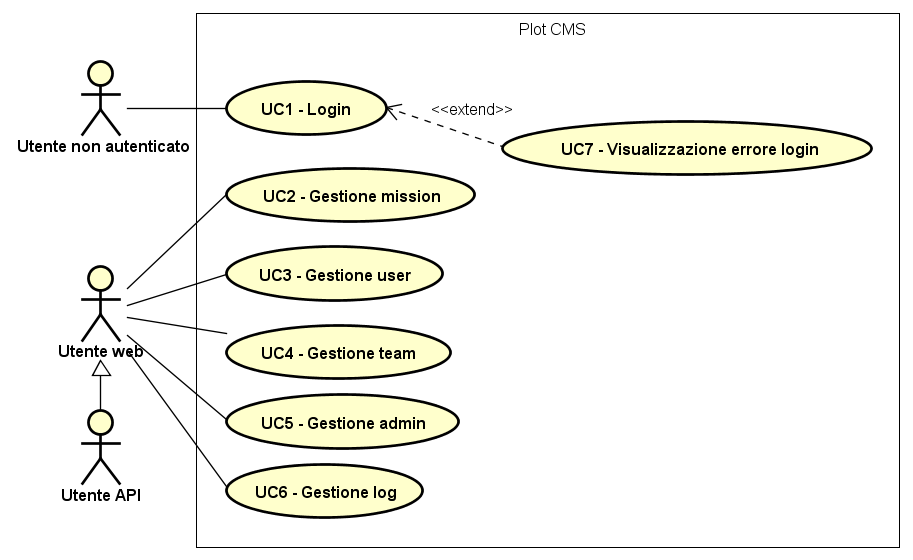
\includegraphics[scale=0.95, width=\textwidth]{immagini/usecase/UCG.png}
            \caption{Caso d'uso UCG: caso d'uso generale}\label{fig:UCG} 
        \end{figure}
\begin{itemize}
\item \textbf{Attori}: utente non autenticato, utente web, utente API;
\item \textbf{Descrizione}: un utente deve poter, innanzitutto, effettuare l'autenticazione presso la piattaforma per poter accedere alle funzionalità offerte.
Una volta effettuata l'autenticazione, l'utente deve poter gestire: mission, amministratori della piattaforma, utenti del gioco, team del gioco e log generati dagli utenti del gioco; 
      \item \textbf{Precondizione}: l'utente accede alla piattaforma attraverso un browser web o attraverso le API REST esposte dal sistema;

        \item \textbf{Flusso principale degli eventi}:
          \begin{enumerate}
          \item L'utente può autenticarsi presso la piattaforma (\hyperlink{UC1}{UC1});
          \item L'utente autenticato può gestire le mission previste dal Plot (\hyperlink{UC2}{UC2});
          \item L'utente autenticato può gestire gli utenti del gioco;
          \item L'utente autenticato può gestire i team del gioco;
          \item L'utente autenticato può gestire gli amministratori della piattaforma;
          \item L'utente autenticato può gestire i log generati dagli utenti del gioco.

      \end{enumerate}
    \item \textbf{Postcondizione}: il sistema ha erogato le funzionalità richieste dall'utente;
     \item \textbf{Scenari alternativi}: 
      \begin{itemize}
       \item Nel caso in cui l'utente provi ad autenticarsi utilizzando una combinazione di username e password non riconosciuta dal sistema: 
       \begin{enumerate}
          \item Viene presentato un errore esplicativo (\hyperlink{UC7}{UC7}).
       \end{enumerate}
      \end{itemize}
  \end{itemize}
\hypertarget{UC1}{}
\subsection{Caso d'uso UC1: login}
\begin{itemize}
\item \textbf{Attori}: utente web;
\item \textbf{Descrizione}: gli amministratori del Plot devono poter autenticarsi presso la piattaforma in modo da poter accedere alle funzionalità offerte; 
      \item \textbf{Precondizione}: l'utente non è già autenticato ed accede alla piattaforma attraverso un browser web o attraverso le API REST esposte dal sistema;

        \item \textbf{Flusso principale degli eventi}:
          \begin{enumerate}
          \item L'utente può inserire una email;
          \item L'utente può inserire una password.

      \end{enumerate}
    \item \textbf{Postcondizione}: l'utente viene riconosciuto dal sistema e può accedere alle funzionalità offerte.
  \end{itemize}
\hypertarget{UC2}{}
\subsection{Caso d'uso UC2: gestione mission}

        \begin{figure}[H]
            \centering
            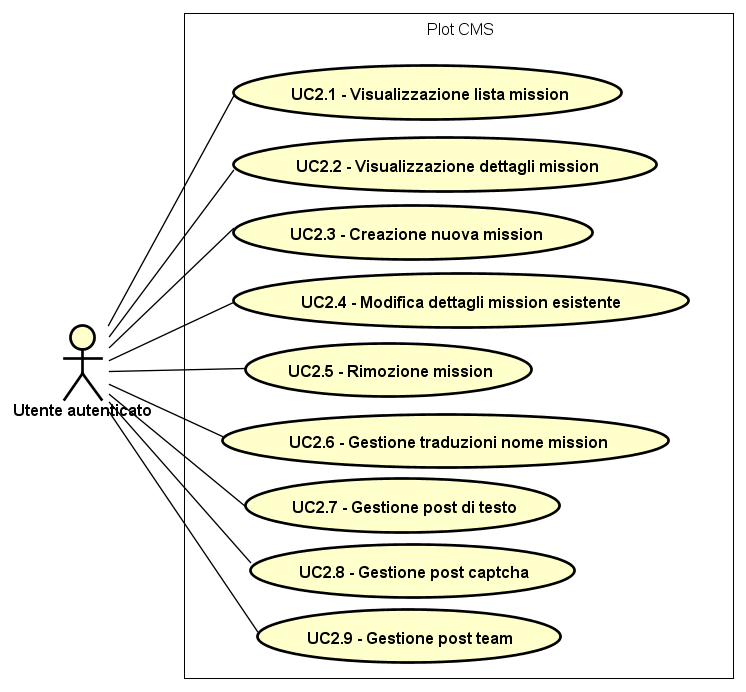
\includegraphics[scale=0.95, width=\textwidth]{immagini/usecase/UC2.png}
            \caption{Caso d'uso UC2: gestione mission}\label{fig:UC2} 
        \end{figure}
\begin{itemize}
\item \textbf{Attori}: utente web, utente API;
\item \textbf{Descrizione}: un utente autenticato deve poter gestire gli aspetti di base legati alle mission: creazione, visualizzazione, modifica e rimozione.
Inoltre deve essere possibile gestire i post legati ad una specifica mission e le traduzioni relative al nome di una specifica mission; 
      \item \textbf{Precondizione}: l'utente accede alla piattaforma attraverso un browser web o attraverso le API REST esposte dal sistema;

        \item \textbf{Flusso principale degli eventi}:
          \begin{enumerate}
          \item L'utente autenticato può visualizzare la lista delle mission;
          \item L'utente autenticato può visualizzare i dettagli di una specifica mission (\hyperlink{UC2.2}{UC2.2});
          \item L'utente autenticato può creare una nuova mission (\hyperlink{UC2.3}{UC2.3});
          \item L'utente autenticato può modificare i dettagli di una specifica mission (\hyperlink{UC2.4}{UC2.4});
          \item L'utente autenticato può rimuovere una mission;
          \item L'utente autenticato può gestire le traduzioni relative al nome di una specifica mission (\hyperlink{UC2.6}{UC2.6});
          \item L'utente autenticato può gestire i post di testo collegati ad una specifica mission (\hyperlink{UC2.7}{UC2.7});
          \item L'utente autenticato può gestire i post di tipo captcha collegati ad una specifica mission (\hyperlink{UC2.8}{UC2.8});
          \item L'utente autenticato può gestire i post di tipo team collegati ad una specifica mission (\hyperlink{UC2.9}{UC2.9}).

      \end{enumerate}
    \item \textbf{Postcondizione}: il sistema ha erogato le funzionalità richieste dall'utente.
  \end{itemize}
\hypertarget{UC2.2}{}
\subsection{Caso d'uso UC2.2: visualizzazione dettagli mission}
\begin{itemize}
\item \textbf{Attori}: utente web, utente API;
\item \textbf{Descrizione}: l'utente autenticato deve poter visualizzare i dettagli relativi ad una specifica mission; 
      \item \textbf{Precondizione}: l'utente accede alla piattaforma attraverso un browser web o attraverso le API REST esposte dal sistema. La mission che si vuole visualizzare deve esistere;

        \item \textbf{Flusso principale degli eventi}:
          \begin{enumerate}
          \item L'utente autenticato visualizza il nome di default della mission;
          \item L'utente autenticato visualizza l'\gls{url}\glsfirstoccur{} dell'immagine rappresentativa della mission;
          \item L'utente autenticato visualizza la data d'inizio della mission;
          \item L'utente autenticato visualizza la data di fine della mission;
          \item L'utente autenticato visualizza il grado di visibilità della mission. Questo indica se la mission è visibile o meno agli utenti di gioco.

      \end{enumerate}
    \item \textbf{Postcondizione}: il sistema mostra all'utente i dettagli della mission richiesta.
  \end{itemize}
\hypertarget{UC2.3}{}
\subsection{Caso d'uso UC2.3: creazione nuova mission}
\begin{itemize}
\item \textbf{Attori}: utente web, utente API;
\item \textbf{Descrizione}: l'utente autenticato deve poter creare una nuova mission; 
      \item \textbf{Precondizione}: l'utente accede alla piattaforma attraverso un browser web o attraverso le API REST esposte dal sistema;

        \item \textbf{Flusso principale degli eventi}:
          \begin{enumerate}
          \item L'utente autenticato inserisce il nome di default della mission;
          \item L'utente autenticato può inserire l'\gls{url}\glsfirstoccur{} di un'immagine rappresentativa della mission;
          \item L'utente autenticato può inserire la data di inizio della mission;
          \item L'utente autenticato può inserire la data di fine della mission;
          \item L'utente autenticato può inserire il grado di visibilità della mission. Questo indica se la mission è visibile o meno agli utenti di gioco.

      \end{enumerate}
    \item \textbf{Postcondizione}: il sistema crea una nuova mission e ne mostra i dettagli all'utente.
  \end{itemize}
\hypertarget{UC2.4}{}
\subsection{Caso d'uso UC2.4: modifica dettagli mission esistente}
\begin{itemize}
\item \textbf{Attori}: utente web, utente API;
\item \textbf{Descrizione}: l'utente autenticato deve poter modificare i dettagli relativi ad una mission esistente; 
      \item \textbf{Precondizione}: l'utente accede alla piattaforma attraverso un browser web o attraverso le API REST esposte dal sistema. La mission che si vuole modificare deve esistere;

        \item \textbf{Flusso principale degli eventi}:
          \begin{enumerate}
          \item L'utente autenticato può modificare il nome di default della mission;
          \item L'utente autenticato può modificare il l'\gls{url}\glsfirstoccur{} dell'immagine rappresentativa della mission;
          \item L'utente autenticato può modificare la data d'inizio della mission;
          \item L'utente autenticato può modificare la data di fine della mission;
          \item L'utente autenticato può modificare il grado di visibilità della mission. Questo indica se la mission è visibile o meno agli utenti di gioco.

      \end{enumerate}
    \item \textbf{Postcondizione}: il sistema apporta le modifiche richieste e mostra i dettagli della mission modificata all'utente.
  \end{itemize}

\hypertarget{UC2.6}{}
\subsection{Caso d'uso UC2.6: gestione traduzioni nome mission}

        \begin{figure}
            \centering
            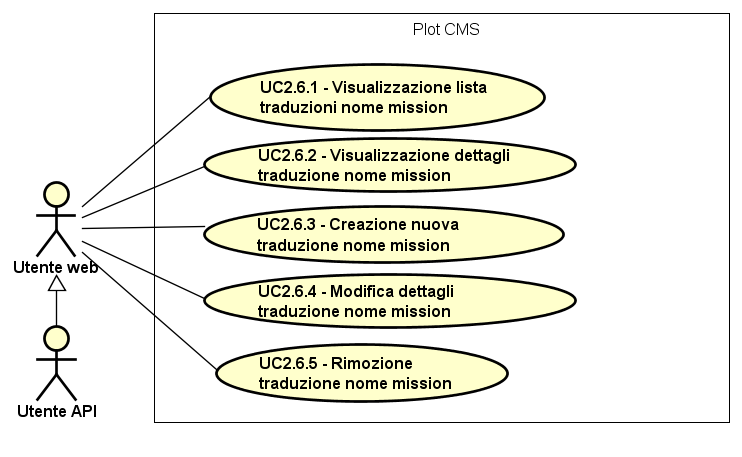
\includegraphics[scale=0.95, width=\textwidth]{immagini/usecase/UC2-6.png}
            \caption{Caso d'uso UC2.6: gestione traduzioni nome mission}\label{fig:UC2.6} 
        \end{figure}
\begin{itemize}
\item \textbf{Attori}: utente web, utente API;
\item \textbf{Descrizione}: un utente autenticato deve poter gestire gli aspetti di base legati alle traduzioni del nome di una mission: creazione, visualizzazione, modifica e rimozione; 
      \item \textbf{Precondizione}: l'utente accede alla piattaforma attraverso un browser web o attraverso le API REST esposte dal sistema;

        \item \textbf{Flusso principale degli eventi}:
          \begin{enumerate}
          \item L'utente autenticato può visualizzare la lista delle traduzioni previste per il nome della mission;
          \item L'utente autenticato può visualizzare i dettagli di una particolare traduzione prevista per il nome della mission (\hyperlink{UC2.6.2}{UC2.6.2});
          \item L'utente autenticato può creare una nuova traduzione per il nome della mission (\hyperlink{UC2.6.3}{UC2.6.3});
          \item L'utente autenticato può modificare i dettagli di una particolare traduzione per il nome della mission (\hyperlink{UC2.6.4}{UC2.6.4});
          \item L'utente autenticato può rimuovere una traduzione relativa al nome della mission.

      \end{enumerate}
    \item \textbf{Postcondizione}: il sistema ha erogato le funzionalità richieste dall'utente.
  \end{itemize}

\hypertarget{UC2.6.2}{}
\subsection{Caso d'uso UC2.6.2: visualizzazione dettagli traduzione nome mission}
\begin{itemize}
\item \textbf{Attori}: utente web, utente API;
\item \textbf{Descrizione}: l'utente autenticato deve poter visualizzare i dettagli relativi ad una specifica traduzione relativa al nome di una mission; 
      \item \textbf{Precondizione}: l'utente accede alla piattaforma attraverso un browser web o attraverso le API REST esposte dal sistema. La traduzione che si vuole visualizzare deve esistere;

        \item \textbf{Flusso principale degli eventi}:
          \begin{enumerate}
          \item L'utente autenticato visualizza la traduzione del nome della mission;
          \item L'utente autenticato visualizza la lingua relativa alla traduzione .

      \end{enumerate}
    \item \textbf{Postcondizione}: il sistema mostra all'utente i dettagli dell'a traduzione richiesta.
  \end{itemize}
\hypertarget{UC2.6.3}{}
\subsection{Caso d'uso UC2.6.3: creazione nuova traduzione nome mission}
\begin{itemize}
\item \textbf{Attori}: utente web, utente API;
\item \textbf{Descrizione}: l'utente autenticato deve poter creare una nuova traduzione relativa al nome della mission. La nuova traduzione è caratterizzata dalla lingua, in quanto non possono esistere due traduzioni fornite nella medesima lingua e riferite al medesimo contenuto; 
      \item \textbf{Precondizione}: l'utente accede alla piattaforma attraverso un browser web o attraverso le API REST esposte dal sistema;

        \item \textbf{Flusso principale degli eventi}:
          \begin{enumerate}
          \item L'utente inserisce il testo della traduzione relativa al nome della mission;
          \item L'utente inserisce la lingua della traduzione relativa al nome della mission.

      \end{enumerate}
    \item \textbf{Postcondizione}: il sistema crea una nuova traduzione e ne mostra i dettagli all'utente.
  \end{itemize}
\hypertarget{UC2.6.4}{}
\subsection{Caso d'uso UC2.6.4: modifica dettagli traduzione nome mission}
\begin{itemize}
\item \textbf{Attori}: utente web, utente API;
\item \textbf{Descrizione}: l'utente autenticato deve poter modificare i dettagli relativi ad una traduzione esistente; 
      \item \textbf{Precondizione}: l'utente accede alla piattaforma attraverso un browser web o attraverso le API REST esposte dal sistema. La traduzione che si vuole modificare deve esistere;

        \item \textbf{Flusso principale degli eventi}:
          \begin{enumerate}
          \item L'utente autenticato può modificare il testo della traduzione relativa al nome della mission;
          \item L'utente autenticato può modificare la lingua della traduzione relativa al nome della mission.

      \end{enumerate}
    \item \textbf{Postcondizione}: il sistema apporta le modifiche richieste e mostra i dettagli della traduzione modificata all'utente.
  \end{itemize}

\hypertarget{UC2.7}{}
\subsection{Caso d'uso UC2.7: gestione post di testo}

        \begin{figure}[H]
            \centering
            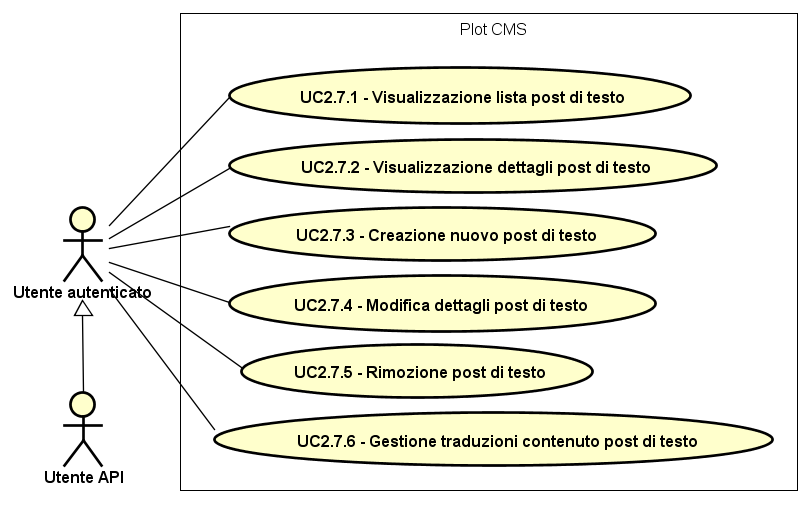
\includegraphics[scale=0.95, width=\textwidth]{immagini/usecase/UC2-7.png}
            \caption{Caso d'uso UC2.7: gestione post di testo}\label{fig:UC2.7} 
        \end{figure}
\begin{itemize}
\item \textbf{Attori}: utente web, utente API;
\item \textbf{Descrizione}: un utente autenticato deve poter gestire gli aspetti di base legati ai post di testo: creazione, visualizzazione, modifica e rimozione. Inoltre deve essere possibile gestire le traduzioni relative al contenuto di uno specifico post di testo. Ogni post di testo è collegato ad una specifica mission; 
      \item \textbf{Precondizione}: l'utente accede alla piattaforma attraverso un browser web o attraverso le API REST esposte dal sistema. I post di testo hanno significato solo come figli di una mission, tale mission deve quindi esistere per poter accedere alle funzionalità di gestione dei post di testo;

        \item \textbf{Flusso principale degli eventi}:
          \begin{enumerate}
          \item L'utente autenticato può visualizzare una lista di tutti i post di testo relativi alla mission;
          \item L'utente autenticato può visualizzare i dettagli di uno specifico post di testo collegato alla mission (\hyperlink{UC2.7.2}{UC2.7.2});
          \item L'utente autenticato può creare un nuovo post di testo collegato alla mission (\hyperlink{UC2.7.3}{UC2.7.3});
          \item L'utente autenticato può modificare i dettagli di un particolare post di testo collegato alla mission (\hyperlink{UC2.7.4}{UC2.7.4});
          \item L'utente autenticato può rimuovere un particolare post di testo collegato alla mission (\hyperlink{UC2.7.5}{UC2.7.5});
          \item L'utente autenticato può gestire le traduzioni del contenuto di un particolare post di testo collegato alla mission (\hyperlink{UC2.7.6}{UC2.7.6}).

      \end{enumerate}
    \item \textbf{Postcondizione}: il sistema ha erogato le funzionalità richieste dall'utente.
  \end{itemize}

\hypertarget{UC2.7.2}{}
\subsection{Caso d'uso UC2.7.2: visualizzazione dettagli post di testo}
\begin{itemize}
\item \textbf{Attori}: utente web, utente API;
\item \textbf{Descrizione}: l'utente autenticato deve poter visualizzare i dettagli relativi ad uno specifico post di testo collegato alla mission; 
      \item \textbf{Precondizione}: l'utente autenticato accede alla piattaforma attraverso un browser web o attraverso le API REST esposte dal sistema. Il post di testo che si vuole visualizzare deve esistere;

        \item \textbf{Flusso principale degli eventi}:
          \begin{enumerate}
          \item L'utente autenticato visualizza il contenuto di default del post di testo;
          \item L'utente autenticato visualizza il grado di visibilità del post di testo. Questo indica se il post è visibile o meno agli utenti di gioco.

      \end{enumerate}
    \item \textbf{Postcondizione}: il sistema mostra all'utente i dettagli del post di testo richiesto.
  \end{itemize}
\hypertarget{UC2.7.3}{}
\subsection{Caso d'uso UC2.7.3: creazione nuovo post di testo}
\begin{itemize}
\item \textbf{Attori}: utente web, utente API;
\item \textbf{Descrizione}: l'utente autenticato deve poter creare un nuovo post di testo, collegandolo alla mission; 
      \item \textbf{Precondizione}: l'utente accede alla piattaforma attraverso un browser web o attraverso le API REST esposte dal sistema;

        \item \textbf{Flusso principale degli eventi}:
          \begin{enumerate}
          \item L'utente autenticato inserisce il contenuto di default del post di testo;
          \item L'utente autenticato inserisce il grado di visibilità del post di testo. Questo indica se il post è visibile o meno agli utenti di gioco.

      \end{enumerate}
    \item \textbf{Postcondizione}: il sistema crea una nuovo post di testo, collegato alla mission, e ne mostra i dettagli all'utente.
  \end{itemize}
\hypertarget{UC2.7.4}{}
\subsection{Caso d'uso UC2.7.4: modifica dettagli post di testo}
\begin{itemize}
\item \textbf{Attori}: utente web, utente API;
\item \textbf{Descrizione}: l'utente autenticato deve poter modificare i dettagli relativi ad un post di testo esistente; 
      \item \textbf{Precondizione}: l'utente accede alla piattaforma attraverso un browser web o attraverso le API REST esposte dal sistema. Il post di testo che si vuole modificare deve esistere;

        \item \textbf{Flusso principale degli eventi}:
          \begin{enumerate}
          \item L'utente autenticato può modificare il contenuto di default del post di testo;
          \item L'utente autenticato può modificare il grado di visibilità del post di testo. Questo indica se il post è visibile o meno agli utenti di gioco.

      \end{enumerate}
    \item \textbf{Postcondizione}: il sistema apporta le modifiche richieste e mostra i dettagli del post di testo modificato all'utente.
  \end{itemize}
\hypertarget{UC2.7.5}{}
\subsection{Caso d'uso UC2.7.5: rimozione post di testo}
\begin{itemize}
\item \textbf{Attori}: utente web, utente API;
\item \textbf{Descrizione}: l'utente autenticato deve poter rimuovere un post di testo; 
      \item \textbf{Precondizione}: l'utente autenticato accede alla piattaforma attraverso un browser web o attraverso le API REST esposte dal sistema. Il post di testo che si vuole rimuovere deve esistere;

        \item \textbf{Flusso principale degli eventi}:
          \begin{enumerate}
          \item L'utente autenticato rimuove un particolare post di testo.

      \end{enumerate}
    \item \textbf{Postcondizione}: Il post di testo viene rimosso dal sistema e non può più essere recuperato. Il sistema mostra all'utente una lista dei post di testo collegati alla mission e ancora presenti nel sistema.
  \end{itemize}
\hypertarget{UC2.7.6}{}
\subsection{Caso d'uso UC2.7.6: gestione traduzioni contenuto post di testo}

        \begin{figure}
            \centering
            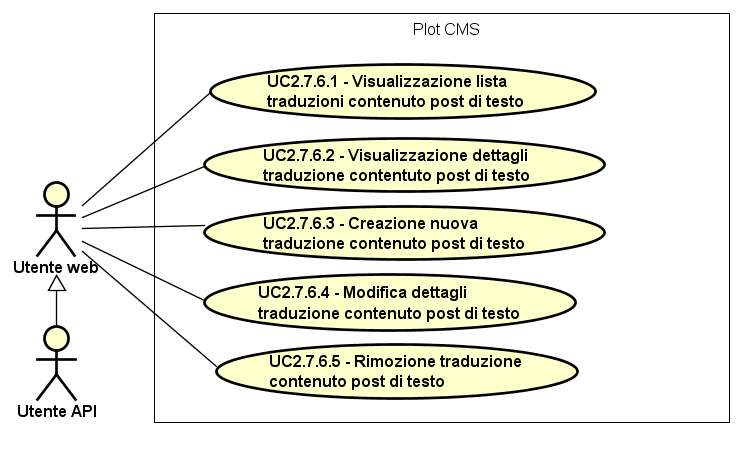
\includegraphics[scale=0.95, width=\textwidth]{immagini/usecase/UC2-7-6.png}
            \caption{Caso d'uso UC2.7.6: gestione traduzioni contenuto post di testo}\label{fig:UC2.7.6} 
        \end{figure}
\begin{itemize}
\item \textbf{Attori}: utente web, utente API;
\item \textbf{Descrizione}: un utente autenticato deve poter gestire gli aspetti di base legati alle traduzioni del contenuto di un post di testo: creazione, visualizzazione, modifica e rimozione; 
      \item \textbf{Precondizione}: l'utente accede alla piattaforma attraverso un browser web o attraverso le API REST esposte dal sistema;

        \item \textbf{Flusso principale degli eventi}:
          \begin{enumerate}
          \item L'utente autenticato può visualizzare la lista delle traduzioni previste per il contenuto del post di testo;
          \item L'utente autenticato può visualizzare i dettagli di una particolare traduzione prevista per il contenuto del post di testo;
          \item L'utente autenticato può creare una nuova traduzione per il contenuto del post di testo;
          \item L'utente autenticato può modificare i dettagli di una particolare traduzione per il contenuto del post di testo;
          \item L'utente autenticato può rimuovere una traduzione relativa al contenuto del post di testo.

      \end{enumerate}
    \item \textbf{Postcondizione}: il sistema ha erogato le funzionalità richieste dall'utente.
  \end{itemize}
\hypertarget{UC2.8}{}
\subsection{Caso d'uso UC2.8: gestione post captcha}

        \begin{figure}
            \centering
            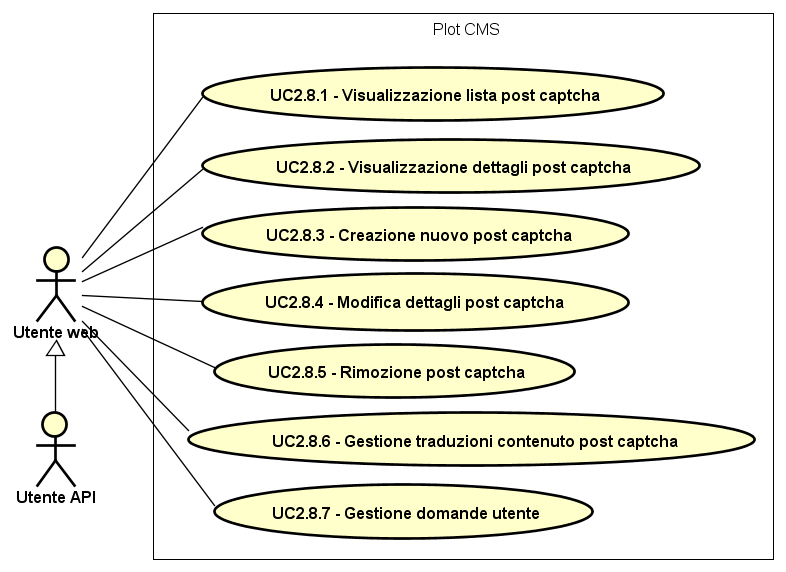
\includegraphics[scale=0.95, width=\textwidth]{immagini/usecase/UC2-8.png}
            \caption{Caso d'uso UC2.8: gestione post captcha}\label{fig:UC2.8} 
        \end{figure}
\begin{itemize}
\item \textbf{Attori}: utente web, utente API;
\item \textbf{Descrizione}: un utente autenticato deve poter gestire gli aspetti di base legati ai post captcha: creazione, visualizzazione, modifica e rimozione. Inoltre deve essere possibile gestire le domande legate ad uno specifico post captcha e le traduzioni relative al contenuto di uno specifico post captcha; 
      \item \textbf{Precondizione}: l'utente accede alla piattaforma attraverso un browser web o attraverso le API REST esposte dal sistema;

        \item \textbf{Flusso principale degli eventi}:
          \begin{enumerate}
          \item L'utente autenticato può visualizzare una lista di tutti i post captcha relativi alla mission;
          \item L'utente autenticato può visualizzare i dettagli di uno specifico post captcha collegato alla mission (\hyperlink{UC2.8.2}{UC2.8.2});
          \item L'utente autenticato può creare un nuovo post captcha collegato alla mission (\hyperlink{UC2.8.3}{UC2.8.3});
          \item L'utente autenticato può modificare i dettagli di un particolare post captcha collegato alla mission (\hyperlink{UC2.8.4}{UC2.8.4});
          \item L'utente autenticato può rimuovere un particolare post captcha collegato alla mission (\hyperlink{UC2.8.5}{UC2.8.5});
          \item L'utente autenticato può gestire le traduzioni del contenuto di un particolare post captcha collegato alla mission (\hyperlink{UC2.8.6}{UC2.8.6});
          \item L'utente autenticato può gestire le domande collegate al post captcha (\hyperlink{UC2.8.7}{UC2.8.7}).

      \end{enumerate}
    \item \textbf{Postcondizione}: il sistema ha erogato le funzionalità richieste dall'utente.
  \end{itemize}

\hypertarget{UC2.8.2}{}
\subsection{Caso d'uso UC2.8.2: visualizzazione dettagli post captcha}
\begin{itemize}
\item \textbf{Attori}: utente web, utente API;
\item \textbf{Descrizione}: l'utente autenticato deve poter visualizzare i dettagli relativi ad uno specifico post captcha collegato alla mission; 
      \item \textbf{Precondizione}: l'utente autenticato accede alla piattaforma attraverso un browser web o attraverso le API REST esposte dal sistema. Il post captcha che si vuole visualizzare deve esistere;

        \item \textbf{Flusso principale degli eventi}:
          \begin{enumerate}
          \item L'utente autenticato visualizza il contenuto di default del post captcha;
          \item L'utente autenticato visualizza il grado di visibilità del post captcha. Questo indica se il post è visibile o meno agli utenti di gioco.

      \end{enumerate}
    \item \textbf{Postcondizione}: il sistema mostra all'utente i dettagli del post captcha richiesto.
  \end{itemize}
\hypertarget{UC2.8.3}{}
\subsection{Caso d'uso UC2.8.3: creazione nuovo post captcha}
\begin{itemize}
\item \textbf{Attori}: utente web, utente API;
\item \textbf{Descrizione}: l'utente autenticato deve poter creare un nuovo post captcha, collegandolo alla mission; 
      \item \textbf{Precondizione}: l'utente accede alla piattaforma attraverso un browser web o attraverso le API REST esposte dal sistema;

        \item \textbf{Flusso principale degli eventi}:
          \begin{enumerate}
          \item L'utente autenticato inserisce il contenuto di default del post captcha;
          \item L'utente autenticato può inserire il grado di visibilità del post captcha. Questo indica se il post è visibile o meno agli utenti di gioco.

      \end{enumerate}
    \item \textbf{Postcondizione}: il sistema crea una nuovo post captcha, collegato alla mission, e ne mostra i dettagli all'utente.
  \end{itemize}
\hypertarget{UC2.8.4}{}
\subsection{Caso d'uso UC2.8.4: modifica dettagli post captcha}
\begin{itemize}
\item \textbf{Attori}: utente web, utente API;
\item \textbf{Descrizione}: l'utente autenticato deve poter modificare i dettagli relativi ad un post captcha esistente; 
      \item \textbf{Precondizione}: l'utente accede alla piattaforma attraverso un browser web o attraverso le API REST esposte dal sistema. Il post captcha che si vuole modificare deve esistere;

        \item \textbf{Flusso principale degli eventi}:
          \begin{enumerate}
          \item L'utente autenticato può modificare il contenuto di default del post captcha;
          \item L'utente autenticato può modificare il grado di visibilità del post captcha. Questo indica se il post è visibile o meno agli utenti di gioco;
          \item L'utente autenticato può modificare il grado di visibilità del post captcha. Questo indica se il post è visibile o meno agli utenti di gioco;
          \item L'utente autenticato può modificare il grado di visibilità del post captcha. Questo indica se il post è visibile o meno agli utenti di gioco.

      \end{enumerate}
    \item \textbf{Postcondizione}: il sistema apporta le modifiche richieste e mostra i dettagli del post captcha modificato all'utente.
  \end{itemize}
\hypertarget{UC2.8.5}{}
\subsection{Caso d'uso UC2.8.5: rimozione post captcha}
\begin{itemize}
\item \textbf{Attori}: utente web, utente API;
\item \textbf{Descrizione}: l'utente autenticato deve poter rimuovere un post captcha; 
      \item \textbf{Precondizione}: l'utente autenticato accede alla piattaforma attraverso un browser web o attraverso le API REST esposte dal sistema. Il post captcha che si vuole rimuovere deve esistere;

        \item \textbf{Flusso principale degli eventi}:
          \begin{enumerate}
          \item L'utente autenticato rimuove un particolare post captcha.

      \end{enumerate}
    \item \textbf{Postcondizione}: Il post captcha viene rimosso dal sistema e non può più essere recuperato. Il sistema mostra all'utente una lista dei post captcha collegati alla mission e ancora presenti nel sistema.
  \end{itemize}
\hypertarget{UC2.8.6}{}
\subsection{Caso d'uso UC2.8.6: gestione traduzioni contenuto post captcha}

        \begin{figure}[H]
            \centering
            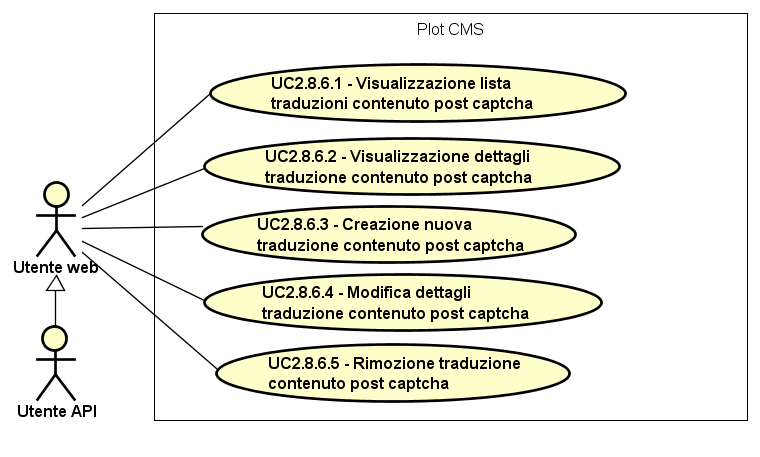
\includegraphics[scale=0.95, width=\textwidth]{immagini/usecase/UC2-8-6.png}
            \caption{Caso d'uso UC2.8.6: gestione traduzioni contenuto post captcha}\label{fig:UC2.8.6} 
        \end{figure}
\begin{itemize}
\item \textbf{Attori}: utente web, utente API;
\item \textbf{Descrizione}: un utente autenticato deve poter gestire gli aspetti di base legati alle traduzioni del contenuto di un post captcha: creazione, visualizzazione, modifica e rimozione; 
      \item \textbf{Precondizione}: l'utente accede alla piattaforma attraverso un browser web o attraverso le API REST esposte dal sistema;

        \item \textbf{Flusso principale degli eventi}:
          \begin{enumerate}
          \item L'utente autenticato può visualizzare la lista delle traduzioni previste per il contenuto del post captcha;
          \item L'utente autenticato può visualizzare i dettagli di una particolare traduzione prevista per il contenuto del post captcha;
          \item L'utente autenticato può creare una nuova traduzione per il contenuto del post captcha;
          \item L'utente autenticato può modificare i dettagli di una particolare traduzione per il contenuto del post captcha;
          \item L'utente autenticato può rimuovere una traduzione relativa al contenuto del post captcha.

      \end{enumerate}
    \item \textbf{Postcondizione}: 	il sistema ha erogato le funzionalità richieste dall'utente.
  \end{itemize}

\hypertarget{UC2.8.7}{}
\subsection{Caso d'uso UC2.8.7: gestione domande utente}

        \begin{figure}[H]
            \centering
            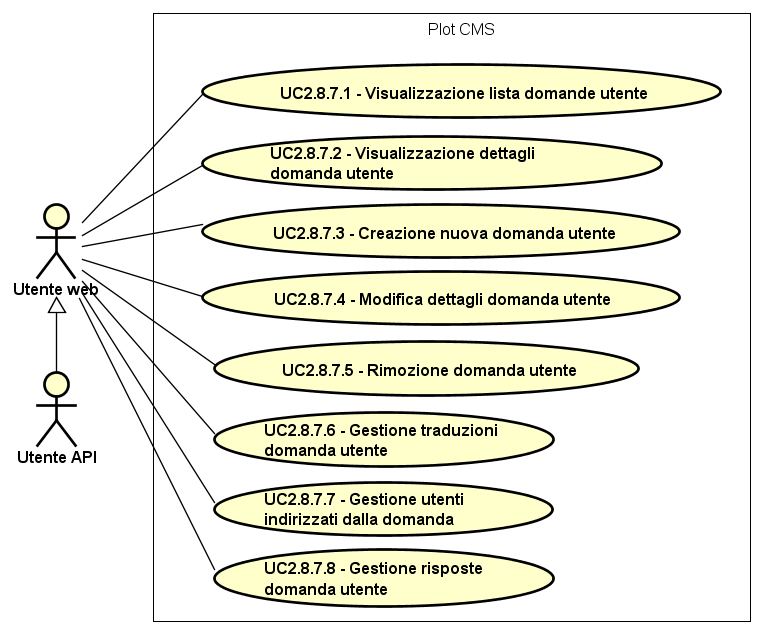
\includegraphics[scale=0.95, width=\textwidth]{immagini/usecase/UC2-8-7.png}
            \caption{Caso d'uso UC2.8.7: gestione domande utente}\label{fig:UC2.8.7} 
        \end{figure}
\begin{itemize}
\item \textbf{Attori}: utente web, utente API;
\item \textbf{Descrizione}: un utente autenticato deve poter gestire gli aspetti di base legati alle domande utente: creazione, visualizzazione, modifica e rimozione.
Inoltre deve essere possibile gestire gli utenti indirizzati dalla domanda e le traduzioni relative ad una specifica domanda.
Le domande utente sono domande rivolte ai singoli utenti del gioco; 
      \item \textbf{Precondizione}: l'utente accede alla piattaforma attraverso un browser web o attraverso le API REST esposte dal sistema. Le domande utente hanno significato solo come figli di un post captcha, tale post deve quindi esistere per poter accedere alle funzionalità di gestione delle domande utente;

        \item \textbf{Flusso principale degli eventi}:
          \begin{enumerate}
          \item L'utente autenticato può visualizzare una lista di tutte le domande collegate ad uno specifico post captcha;
          \item L'utente autenticato può visualizzare i dettagli di una specifica domanda collegata al post captcha (\hyperlink{UC2.8.7.2}{UC2.8.7.2});
          \item L'utente autenticato può creare un nuova domanda collegata al post captcha (\hyperlink{UC2.8.7.3}{UC2.8.7.3});
          \item L'utente autenticato può modificare i dettagli di una particolare domanda collegata al post di tipo captcha (\hyperlink{UC2.8.7.4}{UC2.8.7.4});
          \item L'utente autenticato può rimuovere una particolare domanda collegata al post di tipo captcha (\hyperlink{UC2.8.7.5}{UC2.8.7.5});
          \item L'utente autenticato può gestire le traduzioni della domanda collegata al post di tipo captcha (\hyperlink{UC2.8.7.6}{UC2.8.7.6});
          \item L'utente autenticato può gestire gli utenti indirizzati da una particolare domanda collegata al post di tipo captcha. Gli utenti indirizzati sono coloro ai quali la domanda è rivolta (\hyperlink{UC2.8.7.7}{UC2.8.7.7});
          \item L'utente autenticato può gestire le risposte fornite dagli utenti del gioco ad una specifica domanda utente, collegata ad un post di tipo captcha (\hyperlink{UC2.8.7.8}{UC2.8.7.8}).

      \end{enumerate}
    \item \textbf{Postcondizione}: il sistema ha erogato le funzionalità richieste dall'utente.
  \end{itemize}

\hypertarget{UC2.8.7.2}{}
\subsection{Caso d'uso UC2.8.7.2: visualizzazione dettagli domanda utente}
\begin{itemize}
\item \textbf{Attori}: utente web, utente API;
\item \textbf{Descrizione}: l'utente autenticato deve poter visualizzare i dettagli relativi ad una specifica domanda collegata al post di tipo captcha; 
      \item \textbf{Precondizione}: l'utente autenticato accede alla piattaforma attraverso un browser web o attraverso le API REST esposte dal sistema. La domanda che si vuole visualizzare deve esistere;

        \item \textbf{Flusso principale degli eventi}:
          \begin{enumerate}
          \item L'utente autenticato visualizza il contenuto di default della domanda;
          \item L'utente autenticato visualizza le aree lavorative indirizzare dalla domanda;
          \item L'utente autenticato visualizza le risposte corrette previste per la domanda.

      \end{enumerate}
    \item \textbf{Postcondizione}: il sistema mostra all'utente i dettagli della domanda richiesta.
  \end{itemize}
\hypertarget{UC2.8.7.3}{}
\subsection{Caso d'uso UC2.8.7.3: creazione nuova domanda utente}
\begin{itemize}
\item \textbf{Attori}: utente web, utente API;
\item \textbf{Descrizione}: l'utente autenticato deve poter creare una nuova domanda utente, collegandola ad un post captcha; 
      \item \textbf{Precondizione}: l'utente accede alla piattaforma attraverso un browser web o attraverso le API REST esposte dal sistema;

        \item \textbf{Flusso principale degli eventi}:
          \begin{enumerate}
          \item L'utente autenticato inserisce il contenuto di default della domanda;
          \item L'utente autenticato inserisce le aree lavorative indirizzare dalla domanda;
          \item L'utente autenticato inserisce le risposte corrette previste per la domanda.

      \end{enumerate}
    \item \textbf{Postcondizione}: il sistema crea una nuova domanda utente, collegata al post di tipo captcha, e ne mostra i dettagli all'utente.
  \end{itemize}
\hypertarget{UC2.8.7.4}{}
\subsection{Caso d'uso UC2.8.7.4: modifica dettagli domanda utente}
\begin{itemize}
\item \textbf{Attori}: utente web, utente API;
\item \textbf{Descrizione}: l'utente autenticato deve poter modificare i dettagli relativi ad una domanda utente esistente; 
      \item \textbf{Precondizione}: l'utente accede alla piattaforma attraverso un browser web o attraverso le API REST esposte dal sistema. La domanda che si vuole modificare deve esistere;

        \item \textbf{Flusso principale degli eventi}:
          \begin{enumerate}
          \item L'utente autenticato può modificare il contenuto di default della domanda;
          \item L'utente può modificare le aree lavorative indirizzare dalla domanda;
          \item L'utente autenticato può modificare le risposte corrette previste per la domanda.

      \end{enumerate}
    \item \textbf{Postcondizione}: il sistema apporta le modifiche richieste e mostra i dettagli della domanda modificata all'utente.
  \end{itemize}
\hypertarget{UC2.8.7.5}{}
\subsection{Caso d'uso UC2.8.7.5: rimozione domanda utente}
\begin{itemize}
\item \textbf{Attori}: utente web, utente API;
\item \textbf{Descrizione}: l'utente autenticato deve poter rimuovere una domanda utente; 
      \item \textbf{Precondizione}: l'utente autenticato accede alla piattaforma attraverso un browser web o attraverso le API REST esposte dal sistema. La domanda che si vuole rimuovere deve esistere;

        \item \textbf{Flusso principale degli eventi}:
          \begin{enumerate}
          \item L'utente autenticato rimuove una particolare domanda.

      \end{enumerate}
    \item \textbf{Postcondizione}: la domanda viene rimossa dal sistema e non può più essere recuperata. Il sistema mostra all'utente una lista delle domande utente collegate al post captcha e ancora presenti nel sistema.
  \end{itemize}
\hypertarget{UC2.8.7.6}{}
\subsection{Caso d'uso UC2.8.7.6: gestione traduzioni domanda utente}
\begin{itemize}
\item \textbf{Attori}: utente web, utente API;
\item \textbf{Descrizione}: un utente autenticato deve poter gestire gli aspetti di base legati alle traduzioni del contenuto di una domanda utente: creazione, visualizzazione, modifica e rimozione; 
      \item \textbf{Precondizione}: l'utente accede alla piattaforma attraverso un browser web o attraverso le API REST esposte dal sistema;

        \item \textbf{Flusso principale degli eventi}:
          \begin{enumerate}
          \item L'utente autenticato può visualizzare la lista delle traduzioni previste per il contenuto della domanda utente;
          \item L'utente autenticato può visualizzare i dettagli di una particolare traduzione prevista per il contenuto della domanda utente;
          \item L'utente autenticato può creare una nuova traduzione per il contenuto della domanda utente;
          \item L'utente autenticato può modificare i dettagli di una particolare traduzione per il contenuto della domanda utente;
          \item L'utente autenticato può rimuovere una traduzione relativa al contenuto della domanda utente.

      \end{enumerate}
    \item \textbf{Postcondizione}: il sistema ha erogato le funzionalità richieste dall'utente.
  \end{itemize}
\hypertarget{UC2.8.7.7}{}
\subsection{Caso d'uso UC2.8.7.7: gestione utenti indirizzati dalla domanda}

        \begin{figure}
            \centering
            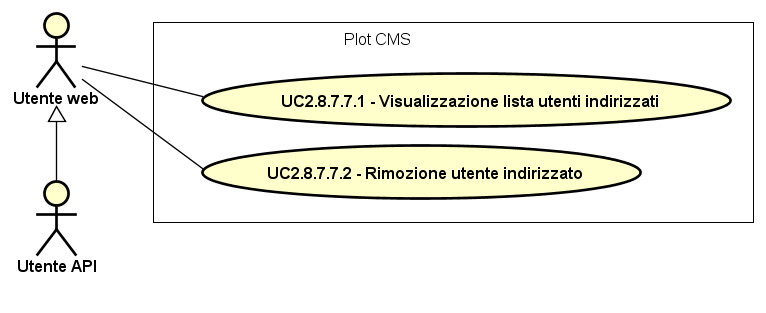
\includegraphics[scale=0.45, width=\textwidth]{immagini/usecase/UC2-8-7-7.png}
            \caption{Caso d'uso UC2.8.7.7: gestione utenti indirizzati dalla domanda}\label{fig:UC2.8.7.7} 
        \end{figure}
\begin{itemize}
\item \textbf{Attori}: utente web, utente API;
\item \textbf{Descrizione}: un utente autenticato deve poter aggiungere, rimuovere e visualizzare gli utenti del gioco ai quali una particolare domanda è rivolta; 
      \item \textbf{Precondizione}: l'utente accede alla piattaforma attraverso un browser web o attraverso le API REST esposte dal sistema. Gli utenti indirizzati hanno significato solo come figli di una domanda utente, tale domanda utente deve quindi esistere ;

        \item \textbf{Flusso principale degli eventi}:
          \begin{enumerate}
          \item L'utente autenticato può visualizzare una lista di tutti gli utenti indirizzati da una specifica domanda, collegata al post captcha;
          \item L'utente autenticato può rimuovere un particolare utente indirizzato dalla domanda (\hyperlink{UC2.8.7.7.2}{UC2.8.7.7.2}).

      \end{enumerate}
    \item \textbf{Postcondizione}: il sistema ha erogato le funzionalità richieste dall'utente.
  \end{itemize}

\hypertarget{UC2.8.7.7.2}{}
\subsection{Caso d'uso UC2.8.7.7.2: rimozione utente indirizzato}
\begin{itemize}
\item \textbf{Attori}: utente web, utente API;
\item \textbf{Descrizione}: l'utente autenticato deve poter rimuovere un utente indirizzato da una specifica domanda. Rimuovere un utente indirizzato non significa rimuovere l'utente di gioco ma rimuovere l'associazione tra l'utente di gioco e la domanda, in modo che la domanda non sia più visibile all'utente di gioco; 
      \item \textbf{Precondizione}: l'utente autenticato accede alla piattaforma attraverso un browser web o attraverso le API REST esposte dal sistema. La utente indirizzato che si vuole rimuovere deve esistere;

        \item \textbf{Flusso principale degli eventi}:
          \begin{enumerate}
          \item L'utente autenticato rimuove un utente indirizzato.

      \end{enumerate}
    \item \textbf{Postcondizione}: l'utente indirizzato viene rimosso dal sistema e non può più essere recuperato. Il sistema mostra all'utente una lista degli utenti di gioco ancora indirizzati dalla domanda.
  \end{itemize}
\hypertarget{UC2.8.7.8}{}
\subsection{Caso d'uso UC2.8.7.8: gestione risposte domanda utente}

        \begin{figure}[H]
            \centering
            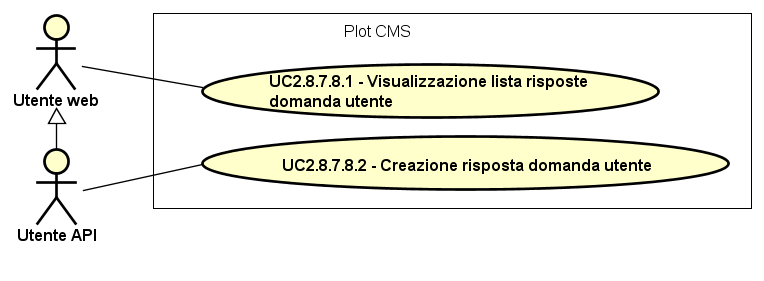
\includegraphics[scale=0.45, width=\textwidth]{immagini/usecase/UC2-8-7-8.png}
            \caption{Caso d'uso UC2.8.7.8: gestione risposte domanda utente}\label{fig:UC2.8.7.8} 
        \end{figure}
\begin{itemize}
\item \textbf{Attori}: utente web, utente API;
\item \textbf{Descrizione}: un utente autenticato deve poter creare e visualizzare le risposte fornite dagli utenti del gioco alle domande ad essi indirizzate; 
      \item \textbf{Precondizione}: l'utente accede alla piattaforma attraverso un browser web o attraverso le API REST esposte dal sistema. Le risposte hanno significato solo come figli di una domanda, tale domanda deve quindi esistere;

        \item \textbf{Flusso principale degli eventi}:
          \begin{enumerate}
          \item l'utente autenticato può visualizzare una lista di tutte le risposte fornite da un utente indirizzato per una specifica domanda utente (\hyperlink{UC2.8.7.8.1}{UC2.8.7.8.1});
          \item l'utente autenticato può creare una nuova risposta, fornita da uno specifico utente indirizzato ad una specifica domanda utente (\hyperlink{UC2.8.7.8.2}{UC2.8.7.8.2}).

      \end{enumerate}
    \item \textbf{Postcondizione}: il sistema ha erogato le funzionalità richieste dall'utente.
  \end{itemize}
\hypertarget{UC2.8.7.8.1}{}
\subsection{Caso d'uso UC2.8.7.8.1: visualizzazione lista risposte domanda utente}
\begin{itemize}
\item \textbf{Attori}: utente web, utente API;
\item \textbf{Descrizione}: l'utente autenticato deve poter visualizzare una lista di tutte le risposte fornite da uno specifico utente indirizzato per una domanda utente. Ogni risposta deve riportare il contenuto della stessa ed un attributo che indichi se è corretta o meno; 
      \item \textbf{Precondizione}: l'utente autenticato accede alla piattaforma attraverso un browser web o attraverso le API REST esposte dal sistema;

        \item \textbf{Flusso principale degli eventi}:
          \begin{enumerate}
          \item l'utente autenticato visualizza la lista delle risposte fornite.

      \end{enumerate}
    \item \textbf{Postcondizione}: il sistema mostra la lista degli utenti di gioco indirizzati dalla domanda.
  \end{itemize}
\hypertarget{UC2.8.7.8.2}{}
\subsection{Caso d'uso UC2.8.7.8.2: creazione risposta domanda utente}
\begin{itemize}
\item \textbf{Attori}: utente API;
\item \textbf{Descrizione}: l'utente autenticato  deve poter creare una nuova risposta fornita da un utente indirizzato per una domanda utente; 
      \item \textbf{Precondizione}: l'utente visualizza la lista degli utenti indirizzati da una specifica domanda;

        \item \textbf{Flusso principale degli eventi}:
          \begin{enumerate}
          \item l'utente autenticato crea una nuova risposta.

      \end{enumerate}
    \item \textbf{Postcondizione}: il sistema mostra la lista degli utenti di gioco indirizzati dalla domanda
.
  \end{itemize}
\hypertarget{UC2.9}{}
\subsection{Caso d'uso UC2.9: gestione post team}

        \begin{figure}[H]
            \centering
            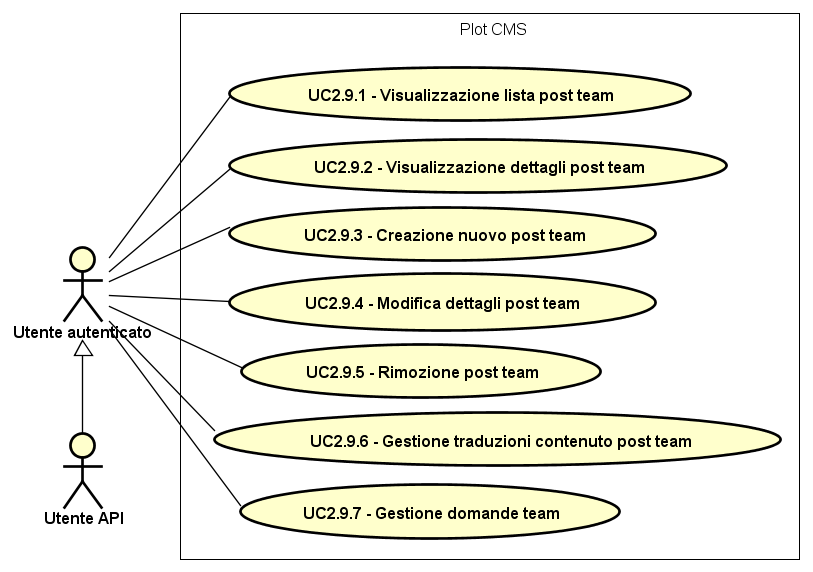
\includegraphics[scale=0.95, width=\textwidth]{immagini/usecase/UC2-9.png}
            \caption{Caso d'uso UC2.9: gestione post team}\label{fig:UC2.9} 
        \end{figure}
\begin{itemize}
\item \textbf{Attori}: utente web, utente API;
\item \textbf{Descrizione}: un utente autenticato deve poter gestire gli aspetti di base legati ai post team: creazione, visualizzazione, modifica e rimozione. Inoltre deve essere possibile gestire le domande legate ad uno specifico post team e le traduzioni relative al contenuto di uno specifico post team; 
      \item \textbf{Precondizione}: l'utente accede alla piattaforma attraverso un browser web o attraverso le API REST esposte dal sistema;

        \item \textbf{Flusso principale degli eventi}:
          \begin{enumerate}
          \item L'utente autenticato può visualizzare una lista di tutti i post team relativi alla mission;
          \item L'utente autenticato può visualizzare i dettagli di uno specifico post team collegato alla mission (\hyperlink{UC2.9.2}{UC2.9.2});
          \item L'utente autenticato può creare un nuovo post team collegato alla mission (\hyperlink{UC2.9.3}{UC2.9.3});
          \item L'utente autenticato può modificare i dettagli di un particolare post team collegato alla mission (\hyperlink{UC2.9.4}{UC2.9.4});
          \item L'utente autenticato può rimuovere un particolare post team collegato alla mission (\hyperlink{UC2.9.5}{UC2.9.5});
          \item L'utente autenticato può gestire le traduzioni del contenuto di un particolare post team collegato alla mission (\hyperlink{UC2.9.6}{UC2.9.6});
          \item L'utente autenticato può gestire le domande collegate al post team (\hyperlink{UC2.9.7}{UC2.9.7}).

      \end{enumerate}
    \item \textbf{Postcondizione}: il sistema ha erogato le funzionalità richieste dall'utente.
  \end{itemize}

\hypertarget{UC2.9.2}{}
\subsection{Caso d'uso UC2.9.2: visualizzazione dettagli post team}
\begin{itemize}
\item \textbf{Attori}: utente web, utente API;
\item \textbf{Descrizione}: l'utente autenticato deve poter visualizzare i dettagli relativi ad uno specifico post team collegato alla mission; 
      \item \textbf{Precondizione}: l'utente autenticato accede alla piattaforma attraverso un browser web o attraverso le API REST esposte dal sistema. Il post team che si vuole visualizzare deve esistere;

        \item \textbf{Flusso principale degli eventi}:
          \begin{enumerate}
          \item L'utente autenticato visualizza il contenuto di default del post team;
          \item L'utente autenticato visualizza il grado di visibilità del post team. Questo indica se il post è visibile o meno agli utenti di gioco;
          \item L'utente autenticato visualizza il tempo limite utile per fornire la risposta corretta alle domande collegate al post .

      \end{enumerate}
    \item \textbf{Postcondizione}: il sistema mostra all'utente i dettagli del post team richiesto.
  \end{itemize}
\hypertarget{UC2.9.3}{}
\subsection{Caso d'uso UC2.9.3: creazione nuovo post team}
\begin{itemize}
\item \textbf{Attori}: utente web, utente API;
\item \textbf{Descrizione}: l'utente autenticato deve poter creare un nuovo post team, collegandolo alla mission; 
      \item \textbf{Precondizione}: l'utente accede alla piattaforma attraverso un browser web o attraverso le API REST esposte dal sistema;

        \item \textbf{Flusso principale degli eventi}:
          \begin{enumerate}
          \item L'utente autenticato inserisce il contenuto di default del post team;
          \item L'utente autenticato può inserire il grado di visibilità del post captcha. Questo indica se il post è visibile o meno agli utenti di gioco;
          \item L'utente autenticato può inserire il tempo limite utile per fornire la risposta corretta alle domande collegate al post.

      \end{enumerate}
    \item \textbf{Postcondizione}: il sistema crea una nuovo post team, collegato alla mission, e ne mostra i dettagli all'utente.
  \end{itemize}
\hypertarget{UC2.9.4}{}
\subsection{Caso d'uso UC2.9.4: modifica dettagli post team}
\begin{itemize}
\item \textbf{Attori}: utente web, utente API;
\item \textbf{Descrizione}: l'utente autenticato deve poter modificare i dettagli relativi ad un post team esistente; 
      \item \textbf{Precondizione}: l'utente accede alla piattaforma attraverso un browser web o attraverso le API REST esposte dal sistema. Il post team che si vuole modificare deve esistere;

        \item \textbf{Flusso principale degli eventi}:
          \begin{enumerate}
          \item L'utente autenticato può modificare il contenuto di default del post team;
          \item L'utente autenticato può modificare il grado di visibilità del post team. Questo indica se il post è visibile o meno agli utenti di gioco;
          \item L'utente autenticato può modificare il tempo limite utile per fornire la risposta corretta alle domande collegate al post.

      \end{enumerate}
    \item \textbf{Postcondizione}: il sistema apporta le modifiche richieste e mostra i dettagli del post team modificato all'utente.
  \end{itemize}
\hypertarget{UC2.9.5}{}
\subsection{Caso d'uso UC2.9.5: rimozione post team}
\begin{itemize}
\item \textbf{Attori}: utente web, utente API;
\item \textbf{Descrizione}: l'utente autenticato deve poter rimuovere un post team; 
      \item \textbf{Precondizione}: l'utente autenticato accede alla piattaforma attraverso un browser web o attraverso le API REST esposte dal sistema. Il post team che si vuole rimuovere deve esistere;

        \item \textbf{Flusso principale degli eventi}:
          \begin{enumerate}
          \item L'utente autenticato rimuove un particolare post team.

      \end{enumerate}
    \item \textbf{Postcondizione}: Il post team viene rimosso dal sistema e non può più essere recuperato. Il sistema mostra all'utente una lista dei post team collegati alla mission e ancora presenti nel sistema.
  \end{itemize}
\hypertarget{UC2.9.6}{}
\subsection{Caso d'uso UC2.9.6: gestione traduzioni contenuto post team}

        \begin{figure}[H]
            \centering
            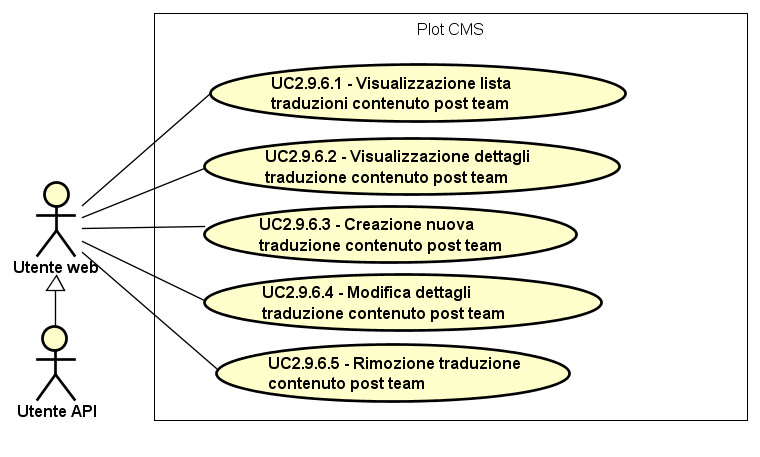
\includegraphics[scale=0.95, width=\textwidth]{immagini/usecase/UC2-9-6.png}
            \caption{Caso d'uso UC2.9.6: gestione traduzioni contenuto post team}\label{fig:UC2.9.6} 
        \end{figure}
\begin{itemize}
\item \textbf{Attori}: utente web, utente API;
\item \textbf{Descrizione}: un utente autenticato deve poter gestire gli aspetti di base legati alle traduzioni del contenuto di un post team: creazione, visualizzazione, modifica e rimozione; 
      \item \textbf{Precondizione}: l'utente accede alla piattaforma attraverso un browser web o attraverso le API REST esposte dal sistema;

        \item \textbf{Flusso principale degli eventi}:
          \begin{enumerate}
          \item L'utente autenticato può visualizzare la lista delle traduzioni previste per il contenuto del post team;
          \item L'utente autenticato può visualizzare i dettagli di una particolare traduzione prevista per il contenuto del post team;
          \item L'utente autenticato può creare una nuova traduzione per il contenuto del post team ;
          \item L'utente autenticato può modificare i dettagli di una particolare traduzione per il contenuto del post team;
          \item L'utente autenticato può rimuovere una traduzione relativa al contenuto del post team.

      \end{enumerate}
    \item \textbf{Postcondizione}: il sistema ha erogato le funzionalità richieste dall'utente.
  \end{itemize}

\hypertarget{UC2.9.7}{}
\subsection{Caso d'uso UC2.9.7: gestione domande team}

        \begin{figure}[H]
            \centering
            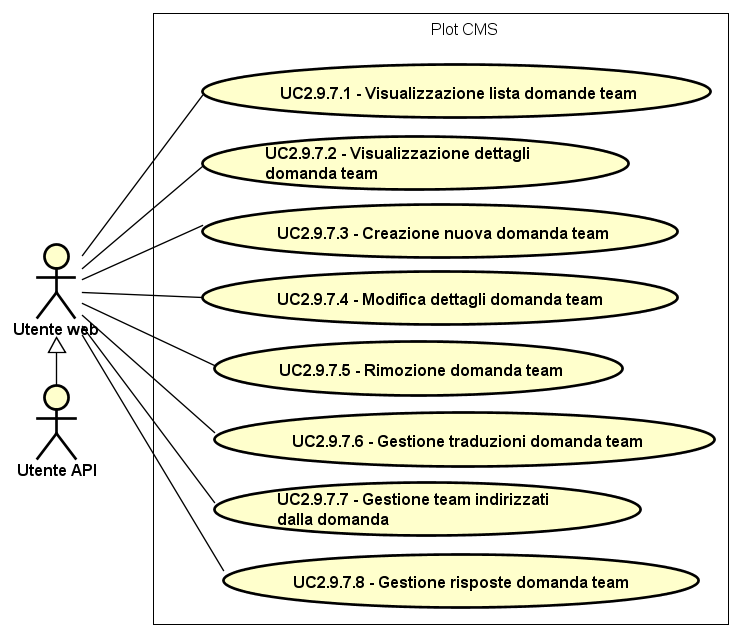
\includegraphics[scale=0.65, width=\textwidth]{immagini/usecase/UC2-9-7.png}
            \caption{Caso d'uso UC2.9.7: gestione domande team}\label{fig:UC2.9.7} 
        \end{figure}
\begin{itemize}
\item \textbf{Attori}: utente web, utente API;
\item \textbf{Descrizione}: un utente autenticato deve poter gestire gli aspetti di base legati alle domande rivolte ai team: creazione, visualizzazione, modifica e rimozione. Inoltre deve essere possibile gestire i team indirizzati dalla domanda e le traduzioni relative ad una specifica domanda; 
      \item \textbf{Precondizione}: l'utente accede alla piattaforma attraverso un browser web o attraverso le API REST esposte dal sistema. Le domande team hanno significato solo come figli di un post team, tale post deve quindi esistere per poter accedere alle funzionalità di gestione delle domande team;

        \item \textbf{Flusso principale degli eventi}:
          \begin{enumerate}
          \item L'utente autenticato può visualizzare una lista di tutte le domande collegate ad uno specifico post team;
          \item L'utente autenticato può visualizzare i dettagli di una specifica domanda collegata al post team (\hyperlink{UC2.9.7.2}{UC2.9.7.2});
          \item L'utente autenticato può creare un nuova domanda collegata al post team (\hyperlink{UC2.9.7.3}{UC2.9.7.3});
          \item L'utente autenticato può modificare i dettagli di una particolare domanda collegata al post di tipo team (\hyperlink{UC2.9.7.4}{UC2.9.7.4});
          \item L'utente autenticato può rimuovere una particolare domanda collegata al post di tipo team (\hyperlink{UC2.9.7.5}{UC2.9.7.5});
          \item L'utente autenticato può gestire le traduzioni della domanda collegata al post di tipo team (\hyperlink{UC2.9.7.6}{UC2.9.7.6});
          \item L'utente autenticato può gestire gli utenti indirizzati da una particolare domanda collegata al post di tipo team. Gli utenti indirizzati sono coloro ai quali la domanda è rivolta (\hyperlink{UC2.9.7.7}{UC2.9.7.7});
          \item L'utente autenticato può gestire le risposte fornite dagli utenti del gioco ad una specifica domanda team, collegata ad un post di tipo team (\hyperlink{UC2.9.7.8}{UC2.9.7.8}).

      \end{enumerate}
    \item \textbf{Postcondizione}: il sistema ha erogato le funzionalità richieste dall'utente.
  \end{itemize}

\hypertarget{UC2.9.7.2}{}
\subsection{Caso d'uso UC2.9.7.2: visualizzazione dettagli domanda team}
\begin{itemize}
\item \textbf{Attori}: utente web, utente API;
\item \textbf{Descrizione}: l'utente autenticato deve poter visualizzare i dettagli relativi ad una specifica domanda collegata al post di tipo team; 
      \item \textbf{Precondizione}: l'utente autenticato accede alla piattaforma attraverso un browser web o attraverso le API REST esposte dal sistema. La domanda che si vuole visualizzare deve esistere;

        \item \textbf{Flusso principale degli eventi}:
          \begin{enumerate}
          \item L'utente autenticato visualizza il contenuto di default della domanda;
          \item L'utente autenticato visualizza le risposte corrette previste per la domanda.

      \end{enumerate}
    \item \textbf{Postcondizione}: il sistema mostra all'utente i dettagli della domanda richiesta.
  \end{itemize}
\hypertarget{UC2.9.7.3}{}
\subsection{Caso d'uso UC2.9.7.3: creazione nuova domanda team}
\begin{itemize}
\item \textbf{Attori}: utente web, utente API;
\item \textbf{Descrizione}: l'utente autenticato deve poter creare una nuova domanda team, collegandola ad un post di tipo team; 
      \item \textbf{Precondizione}: l'utente accede alla piattaforma attraverso un browser web o attraverso le API REST esposte dal sistema;

        \item \textbf{Flusso principale degli eventi}:
          \begin{enumerate}
          \item L'utente autenticato inserisce il contenuto di default della domanda;
          \item L'utente autenticato inserisce le risposte corrette previste per la domanda.

      \end{enumerate}
    \item \textbf{Postcondizione}: il sistema crea una nuova domanda collegata al post di tipo team, e ne mostra i dettagli all'utente.
  \end{itemize}
\hypertarget{UC2.9.7.4}{}
\subsection{Caso d'uso UC2.9.7.4: modifica dettagli domanda team}
\begin{itemize}
\item \textbf{Attori}: utente web, utente API;
\item \textbf{Descrizione}: l'utente autenticato deve poter modificare i dettagli relativi ad una domanda di tipo team esistente; 
      \item \textbf{Precondizione}: l'utente accede alla piattaforma attraverso un browser web o attraverso le API REST esposte dal sistema. La domanda che si vuole modificare deve esistere;

        \item \textbf{Flusso principale degli eventi}:
          \begin{enumerate}
          \item L'utente autenticato può modificare il contenuto di default della domanda;
          \item L'utente autenticato può modificare le risposte corrette previste per la domanda.

      \end{enumerate}
    \item \textbf{Postcondizione}: il sistema apporta le modifiche richieste e mostra i dettagli della domanda modificata all'utente.
  \end{itemize}
\hypertarget{UC2.9.7.5}{}
\subsection{Caso d'uso UC2.9.7.5: rimozione domanda team}
\begin{itemize}
\item \textbf{Attori}: utente web, utente API;
\item \textbf{Descrizione}: l'utente autenticato deve poter rimuovere una domanda di tipo team; 
      \item \textbf{Precondizione}: 'utente autenticato accede alla piattaforma attraverso un browser web o attraverso le API REST esposte dal sistema. La domanda che si vuole rimuovere deve esistere;

        \item \textbf{Flusso principale degli eventi}:
          \begin{enumerate}
          \item L'utente autenticato rimuove una particolare domanda.

      \end{enumerate}
    \item \textbf{Postcondizione}: la domanda viene rimossa dal sistema e non può più essere recuperata. Il sistema mostra all'utente una lista delle domande collegate al post di tipo team ancora presenti nel sistema.
  \end{itemize}
\hypertarget{UC2.9.7.6}{}
\subsection{Caso d'uso UC2.9.7.6: gestione traduzioni domanda team}
\begin{itemize}
\item \textbf{Attori}: utente web, utente API;
\item \textbf{Descrizione}: un utente autenticato deve poter gestire gli aspetti di base legati alle traduzioni del contenuto di una domanda di tipo team: creazione, visualizzazione, modifica e rimozione; 
      \item \textbf{Precondizione}: l'utente accede alla piattaforma attraverso un browser web o attraverso le API REST esposte dal sistema;

        \item \textbf{Flusso principale degli eventi}:
          \begin{enumerate}
          \item L'utente autenticato può visualizzare la lista delle traduzioni previste per il contenuto della domanda di tipo team;
          \item L'utente autenticato può visualizzare i dettagli di una particolare traduzione prevista per il contenuto della domanda di tipo team;
          \item 'utente autenticato può creare una nuova traduzione per il contenuto della domanda di tipo team;
          \item L'utente autenticato può modificare i dettagli di una particolare traduzione per il contenuto della domanda di tipo team;
          \item L'utente autenticato può rimuovere una traduzione relativa al contenuto della domanda di tipo team.

      \end{enumerate}
    \item \textbf{Postcondizione}: il sistema ha erogato le funzionalità richieste dall'utente.
  \end{itemize}
\hypertarget{UC2.9.7.7}{}
\subsection{Caso d'uso UC2.9.7.7: gestione team indirizzati dalla domanda}

        \begin{figure}[H]
            \centering
            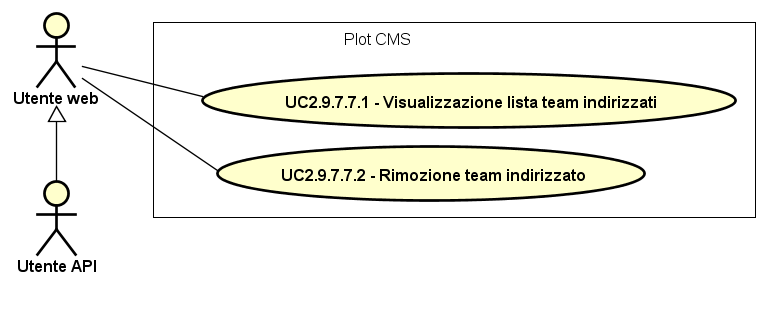
\includegraphics[scale=0.65, width=\textwidth]{immagini/usecase/UC2-9-7-7.png}
            \caption{Caso d'uso UC2.9.7.7: gestione team indirizzati dalla domanda}\label{fig:UC2.9.7.7} 
        \end{figure}
\begin{itemize}
\item \textbf{Attori}: utente web, utente API;
\item \textbf{Descrizione}: un utente autenticato deve poter aggiungere, rimuovere e visualizzare i team ai quali una particolare domanda è rivolta; 
      \item \textbf{Precondizione}: l'utente accede alla piattaforma attraverso un browser web o attraverso le API REST esposte dal sistema. I team indirizzati hanno significato solo come figli di una domanda di tipo team, tale domanda deve quindi esistere;

        \item \textbf{Flusso principale degli eventi}:
          \begin{enumerate}
          \item L'utente autenticato può visualizzare una lista di tutti i team indirizzati da una specifica domanda, collegata al post di tipo team (\hyperlink{UC2.9.7.7.1}{UC2.9.7.7.1});
          \item L'utente autenticato può rimuovere un particolare team indirizzato dalla domanda (\hyperlink{UC2.9.7.7.2}{UC2.9.7.7.2}).

      \end{enumerate}
    \item \textbf{Postcondizione}: il sistema ha erogato le funzionalità richieste dall'utente.
  \end{itemize}
\hypertarget{UC2.9.7.7.1}{}
\subsection{Caso d'uso UC2.9.7.7.1: visualizzazione lista team indirizzati}
\begin{itemize}
\item \textbf{Attori}: utente web, utente API;
\item \textbf{Descrizione}: l'utente autenticato deve poter visualizzare una lista di tutti i team ai quali una specifica domanda (collegata ad un post di tipo team) è rivolta; 
      \item \textbf{Precondizione}: l'utente autenticato accede alla piattaforma attraverso un browser web o attraverso le API REST esposte dal sistema;

        \item \textbf{Flusso principale degli eventi}:
          \begin{enumerate}
          \item l'utente visualizza la lista dei team indirizzati da una specifica domanda.

      \end{enumerate}
    \item \textbf{Postcondizione}: il sistema mostra la lista dei team indirizzati dalla domanda.
  \end{itemize}
\hypertarget{UC2.9.7.7.2}{}
\subsection{Caso d'uso UC2.9.7.7.2: rimozione team indirizzato}
\begin{itemize}
\item \textbf{Attori}: utente web, utente API;
\item \textbf{Descrizione}: l'utente autenticato deve poter rimuovere un team indirizzato da una specifica domanda. Rimuovere un team indirizzato non significa rimuovere il team dal gioco ma rimuovere l'associazione tra il team e la domanda, in modo che la domanda non sia più visibile la team; 
      \item \textbf{Precondizione}: l'utente autenticato accede alla piattaforma attraverso un browser web o attraverso le API REST esposte dal sistema. Il team indirizzato che si vuole rimuovere deve esistere;

        \item \textbf{Flusso principale degli eventi}:
          \begin{enumerate}
          \item L'utente autenticato rimuove un team indirizzato.

      \end{enumerate}
    \item \textbf{Postcondizione}: il team indirizzato viene rimosso dal sistema e non può più essere recuperato. Il sistema mostra all'utente una lista dei team ancora indirizzati dalla domanda.
  \end{itemize}
\hypertarget{UC2.9.7.8}{}
\subsection{Caso d'uso UC2.9.7.8: gestione risposte domanda team}

        \begin{figure}[H]
            \centering
            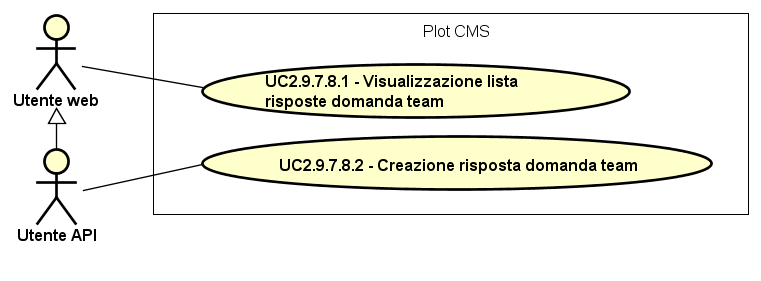
\includegraphics[scale=0.65, width=\textwidth]{immagini/usecase/UC2-9-7-8.png}
            \caption{Caso d'uso UC2.9.7.8: gestione risposte domanda team}\label{fig:UC2.9.7.8} 
        \end{figure}
\begin{itemize}
\item \textbf{Attori}: utente web, utente API;
\item \textbf{Descrizione}: un utente autenticato deve poter creare e visualizzare le risposte fornite dai team alle domande ad essi indirizzate; 
      \item \textbf{Precondizione}: l'utente accede alla piattaforma attraverso un browser web o attraverso le API REST esposte dal sistema. Le risposte hanno significato solo come figli di una domanda, tale domanda deve quindi esistere;

        \item \textbf{Flusso principale degli eventi}:
          \begin{enumerate}
          \item l'utente autenticato può visualizzare una lista di tutte le risposte fornite da un team indirizzato per una specifica domanda di tipo team (\hyperlink{UC2.9.7.8.1}{UC2.9.7.8.1});
          \item l'utente autenticato può creare una nuova risposta, fornita da uno specifico team indirizzato ad una specifica domanda udi tipo team (\hyperlink{UC2.9.7.8.2}{UC2.9.7.8.2}).

      \end{enumerate}
    \item \textbf{Postcondizione}: il sistema ha erogato le funzionalità richieste dall'utente.
  \end{itemize}
\hypertarget{UC2.9.7.8.1}{}
\subsection{Caso d'uso UC2.9.7.8.1: visualizzazione lista risposte domanda team}
\begin{itemize}
\item \textbf{Attori}: utente web, utente API;
\item \textbf{Descrizione}: l'utente autenticato deve poter visualizzare una lista di tutte le risposte fornite da uno specifico team indirizzato per una domanda di tipo team. Ogni risposta deve riportare il contenuto della stessa ed un attributo che indichi se è corretta o meno; 
      \item \textbf{Precondizione}: 	l'utente autenticato accede alla piattaforma attraverso un browser web o attraverso le API REST esposte dal sistema;

        \item \textbf{Flusso principale degli eventi}:
          \begin{enumerate}
          \item l'utente autenticato visualizza la lista delle risposte fornite.

      \end{enumerate}
    \item \textbf{Postcondizione}: il sistema mostra la lista degli utenti di gioco indirizzati dalla domanda.
  \end{itemize}
\hypertarget{UC2.9.7.8.2}{}
\subsection{Caso d'uso UC2.9.7.8.2: creazione risposta domanda team}
\begin{itemize}
\item \textbf{Attori}: utente API;
\item \textbf{Descrizione}: l'utente autenticato deve poter creare una nuova risposta fornita da un team indirizzato per una domanda udi tipo team; 
      \item \textbf{Precondizione}: l'utente visualizza la lista degli utenti indirizzati da una specifica domanda;

        \item \textbf{Flusso principale degli eventi}:
          \begin{enumerate}
          \item l'utente autenticato crea una nuova risposta.

      \end{enumerate}
    \item \textbf{Postcondizione}: il sistema mostra la lista dei team in gioco indirizzati dalla domanda.
  \end{itemize}

\hypertarget{UC7}{}
\subsection{Caso d'uso UC7: visualizzazione errore login}
\begin{itemize}
\item \textbf{Attori}: utente non autenticato;
\item \textbf{Descrizione}: viene visualizzato un messaggio d'errore ad indicare che l'autenticazione dell'utente non è andata a buon fine. Questo può accadere nel caso in cui l'utente inserisca delle credenziali non riconosciute dal sistema; 
      \item \textbf{Precondizione}: l'utente non è già autenticato, accede alla piattaforma e utilizza delle credenziali non riconosciute per autenticarsi al sistema;

        \item \textbf{Flusso principale degli eventi}:
          \begin{enumerate}
          \item L'utente visualizza un messaggio d'errore relativo alla fallita autenticazione.

      \end{enumerate}
    \item \textbf{Postcondizione}: il messaggio d'errore viene mostrato all'utente.
  \end{itemize}
 
